%-------------------------------------------------------------------------------
%   Haskellerのための圏論
%   Keichi
%   圏論の勉強成果の個人的なまとめ
%-------------------------------------------------------------------------------

%-------------------------------------------------------------------------------
\newpage
\section{関手}

\subsection{定義}
$C$, $D$を圏とすると、関手(Functor)$F:C \to D$は
関数$F_{objects}:Ob(C) \to Ob(D)$と関数$F_{arrows}:Ar(C)\to Ar(D)$の組である。
前者は対象関数とよばれ、後者は射関数とよばれる。

\begin{figure}[htbp]
    \centering
    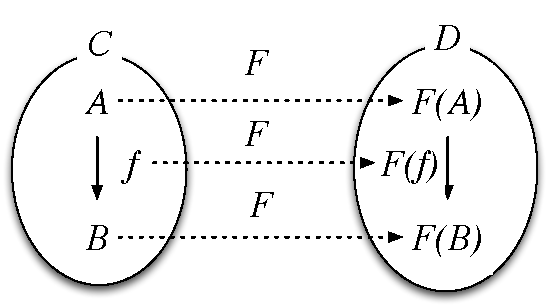
\includegraphics{diag_functor.pdf}
    \caption{関手$F$}
\end{figure}

\subsection{公理}
\begin{itemize}
    \item 圏$C$において$f:A\to B$が存在すれば、
        圏$D$において$F(f):F(A)\to F(B)$である
    \item 圏$C$において$g:B\to C$、$f:A\to B$が存在すれば、
        $F(f)\circ F(g)=F(f\circ g)$が成り立つ
    \item 圏$C$の全ての対象について、$id_{F(A)}=F(id_A)$
\end{itemize}

\subsection{Haskellにおける関手}
厳密には、Haskell圏における関手は、Haskellの型と関数に対するあらゆる操作うち、
上記の公理を満たすものである。しかし、Haskellはプログラミング言語であるので、
実際Haskellで扱うのは、対象関数と射関数の両方がHaskellで書ける関手だけである。
具体的には、Haskellにおける関手の対象関数は、
多くの場合データコンストラクタであり、射関数は多相関数fmapとなる。
これは型クラスFunctorで宣言されている:

\begin{lstlisting}
class Functor f where
    fmap :: (a -> b) -> (f a -> f b)
\end{lstlisting}

Haskellにおいて、ListやMaybe、Treeなどは全てFunctorクラスの
インスタンスであり、Functorクラスのインスタンスは以下の条件
\begin{lstlisting}
    fmap id = id
    fmap f . fmap g = fmap (f . g)
\end{lstlisting}
を満たすべきであるとされている。これは上記の公理に相当する。

具体的な例として、Hask圏からMaybe圏への関手Maybeを考える。
関手Maybeの対象関数はJustであり、射関数はfmapとなる。
\begin{lstlisting}
    --元の圏の上での関数f
    f :: Int -> Int
    f x =  x * x

    --fをMaybeの圏の射に写像する
    g :: Maybe Int -> Maybe Int
    g = fmap f

    --元の圏の上での値
    a = 3
    --aをMaybeの圏の対象に写像する
    b = Just a

    main = do
        --元の圏の上で対象に射を適用
        print $ f a
        --Maybeの圏の上で対象に射を適用
        print $ g b
\end{lstlisting}


%-------------------------------------------------------------------------------
